\documentclass[11pt]{article}
\usepackage{geometry}                
\geometry{letterpaper}                   





\usepackage[english]{babel}
\usepackage[utf8x]{inputenc}
\usepackage{amsmath}
\usepackage{tikz}
\usetikzlibrary{positioning}

\usetikzlibrary{arrows,automata}


%\usepackage[latin1]{inputenc}
\usepackage{graphicx}
\usepackage{amssymb}
\usepackage{epstopdf}
\usepackage{natbib}
\usepackage{amssymb, amsmath}
\DeclareGraphicsRule{.tif}{png}{.png}{`convert #1 `dirname #1`/`basename #1 .tif`.png}
\title{Airplane Boarding}
\author{Anton Schäfer, Nils Blach}
%\date{date} 

\begin{document}



\thispagestyle{empty}

\begin{center}
\includegraphics[width=5cm]{ETHlogo.eps}

\bigskip


\bigskip


\bigskip


\LARGE{ 	Lecture with Computer Exercises:\\ }
\LARGE{ Modelling and Simulating Social Systems\\}

\bigskip

\bigskip

\small{Project Report}\\

\bigskip

\bigskip

\bigskip

\bigskip


\begin{tabular}{|c|}
\hline
\\
\textbf{\LARGE{Insert Title Here}}\\
\textbf{\LARGE{...}}\\
\\
\hline
\end{tabular}
\bigskip

\bigskip

\bigskip

\LARGE{Name 1, Name 2  \& [...]}



\bigskip

\bigskip

\bigskip

\bigskip

\bigskip

\bigskip

\bigskip

\bigskip

Zurich\\
Dec 2018\\

\end{center}



\newpage

%%%%%%%%%%%%%%%%%%%%%%%%%%%%%%%%%%%%%%%%%%%%%%%%%

\newpage
\section*{Agreement for free-download}
\bigskip


\bigskip


\large We hereby agree to make our source code for this project freely available for download from the web pages of COSS. Furthermore, we assure that all source code is written by ourselves and is not violating any copyright restrictions.

\begin{center}

\bigskip


\bigskip


\begin{tabular}{@{}p{3.3cm}@{}p{6cm}@{}@{}p{6cm}@{}}
\begin{minipage}{3cm}

\end{minipage}
&
\begin{minipage}{6cm}
	\vspace{2mm} \large Anton Sch{\"a}fer

 \vspace{\baselineskip}

\end{minipage}
&
\begin{minipage}{6cm}

\large Nils Blach

\end{minipage}
\end{tabular}


\end{center}
\newpage

%%%%%%%%%%%%%%%%%%%%%%%%%%%%%%%%%%%%%%%



% IMPORTANT
% you MUST include the ETH declaration of originality here; it is available for download on the course website or at http://www.ethz.ch/faculty/exams/plagiarism/index_EN; it can be printed as pdf and should be filled out in handwriting


%%%%%%%%%% Table of content %%%%%%%%%%%%%%%%%

\tableofcontents

\newpage

%%%%%%%%%%%%%%%%%%%%%%%%%%%%%%%%%%%%%%%



\section{Abstract}

\section{Individual contributions}
\paragraph{Model:} Both
\paragraph{Data Collection/Calculation:} Anton Sch{\"a}fer
\paragraph{Data Display/Graphs:} Nils Blach

\section{Introduction and Motivations}

\section{Description of the Model}

\begin{figure}
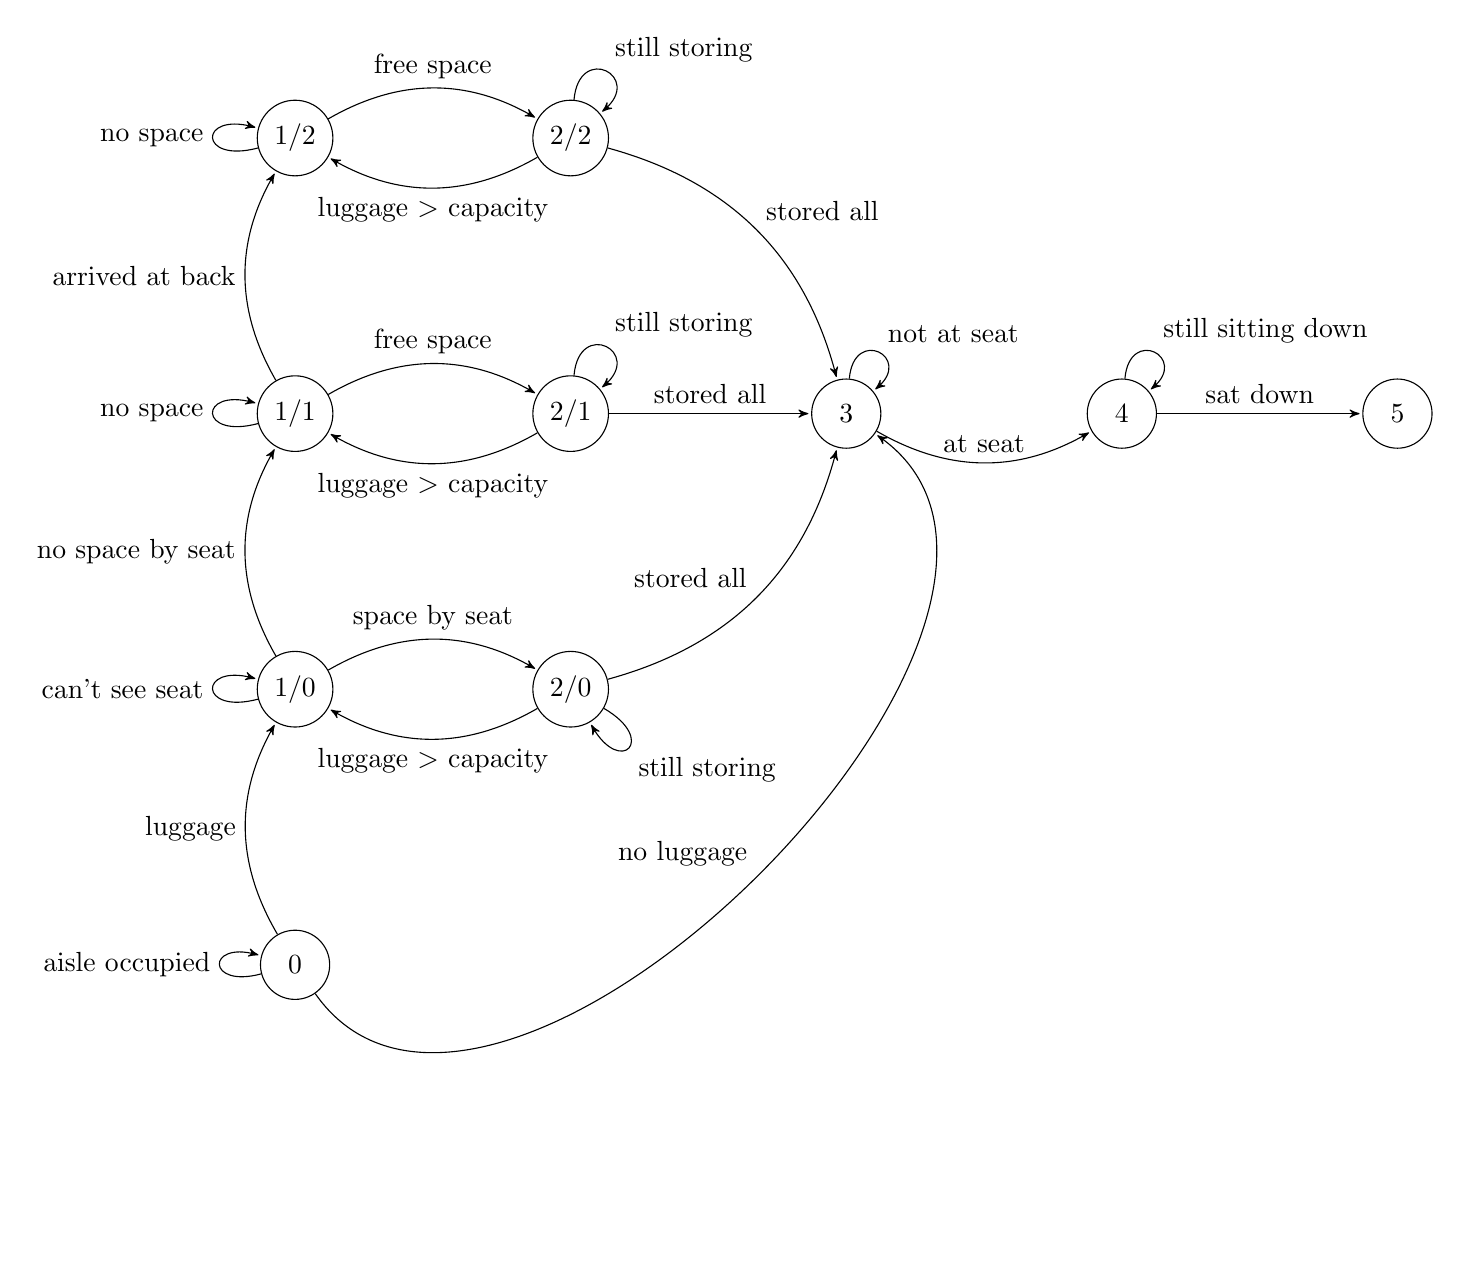
\begin{tikzpicture}[->,>=stealth',shorten >=1pt,auto,node distance=3.5cm,
        scale = 1,transform shape]

  \node[state] (0) [] {$0$};
  \node[state] (1/0) [above of=0] {$1/0$};
  \node[state] (1/1) [above of=1/0] {$1/1$};
  \node[state] (1/2) [above of=1/1] {$1/2$};
  \node[state] (2/0) [right of=1/0] {$2/0$};
  \node[state] (2/1) [right of=1/1] {$2/1$};
  \node[state] (2/2) [right of=1/2] {$2/2$};
  \node[state] (3) [right of=2/1] {$3$};
  \node[state] (4) [right of=3] {$4$};
  \node[state] (5) [right of=4] {$5$};

  \path (0) edge   [bend left]           node {luggage} (1/0)
        (0) edge  [bend right=100]            node {no luggage} (3)
        (0) edge  [loop left]            node {aisle occupied} (0)
        (1/0) edge  [loop left]            node {can't see seat} (1/0)
        (1/0) edge    [bend left]          node {no space by seat} (1/1)
        (1/0) edge   [bend left]           node {space by seat} (2/0)
        (1/1) edge  [loop left]            node {no space} (1/1)
        (1/1) edge   [bend left]           node {arrived at back} (1/2)
        (1/1) edge   [bend left]            node {free space} (2/1)
        (1/2) edge   [loop left]           node {no space} (1/2)
        (1/2) edge    [bend left]           node {free space} (2/2)
        (2/0) edge     [out=330,in=300,looseness=8]        node {still storing} (2/0)
        (2/0) edge    [bend left]          node {luggage $>$ capacity} (1/0)
        (2/0) edge     [bend right]         node {stored all} (3)
        (2/1) edge      [out=85,in=40,looseness=5]        node {still storing} (2/1)
        (2/1) edge     [bend left]         node {luggage $>$ capacity} (1/1)
        (2/1) edge              node {stored all} (3)
        (2/2) edge     [out=85,in=40,looseness=5]         node {still storing} (2/2)
        (2/2) edge     [bend left]         node {luggage $>$ capacity} (1/2)
        (2/2) edge     [bend left]         node {stored all} (3)
        (3) edge     [out=85,in=40,looseness=5]       node {not at seat} (3)
        (3) edge     [bend right]         node {at seat} (4)
        (4) edge      [out=85,in=40,looseness=5]         node {still sitting down} (4)
        (4) edge              node {sat down} (5);

\end{tikzpicture}
\end{figure}
 


\section{Implementation}

\section{Simulation Results and Discussion}
\begin{figure}
	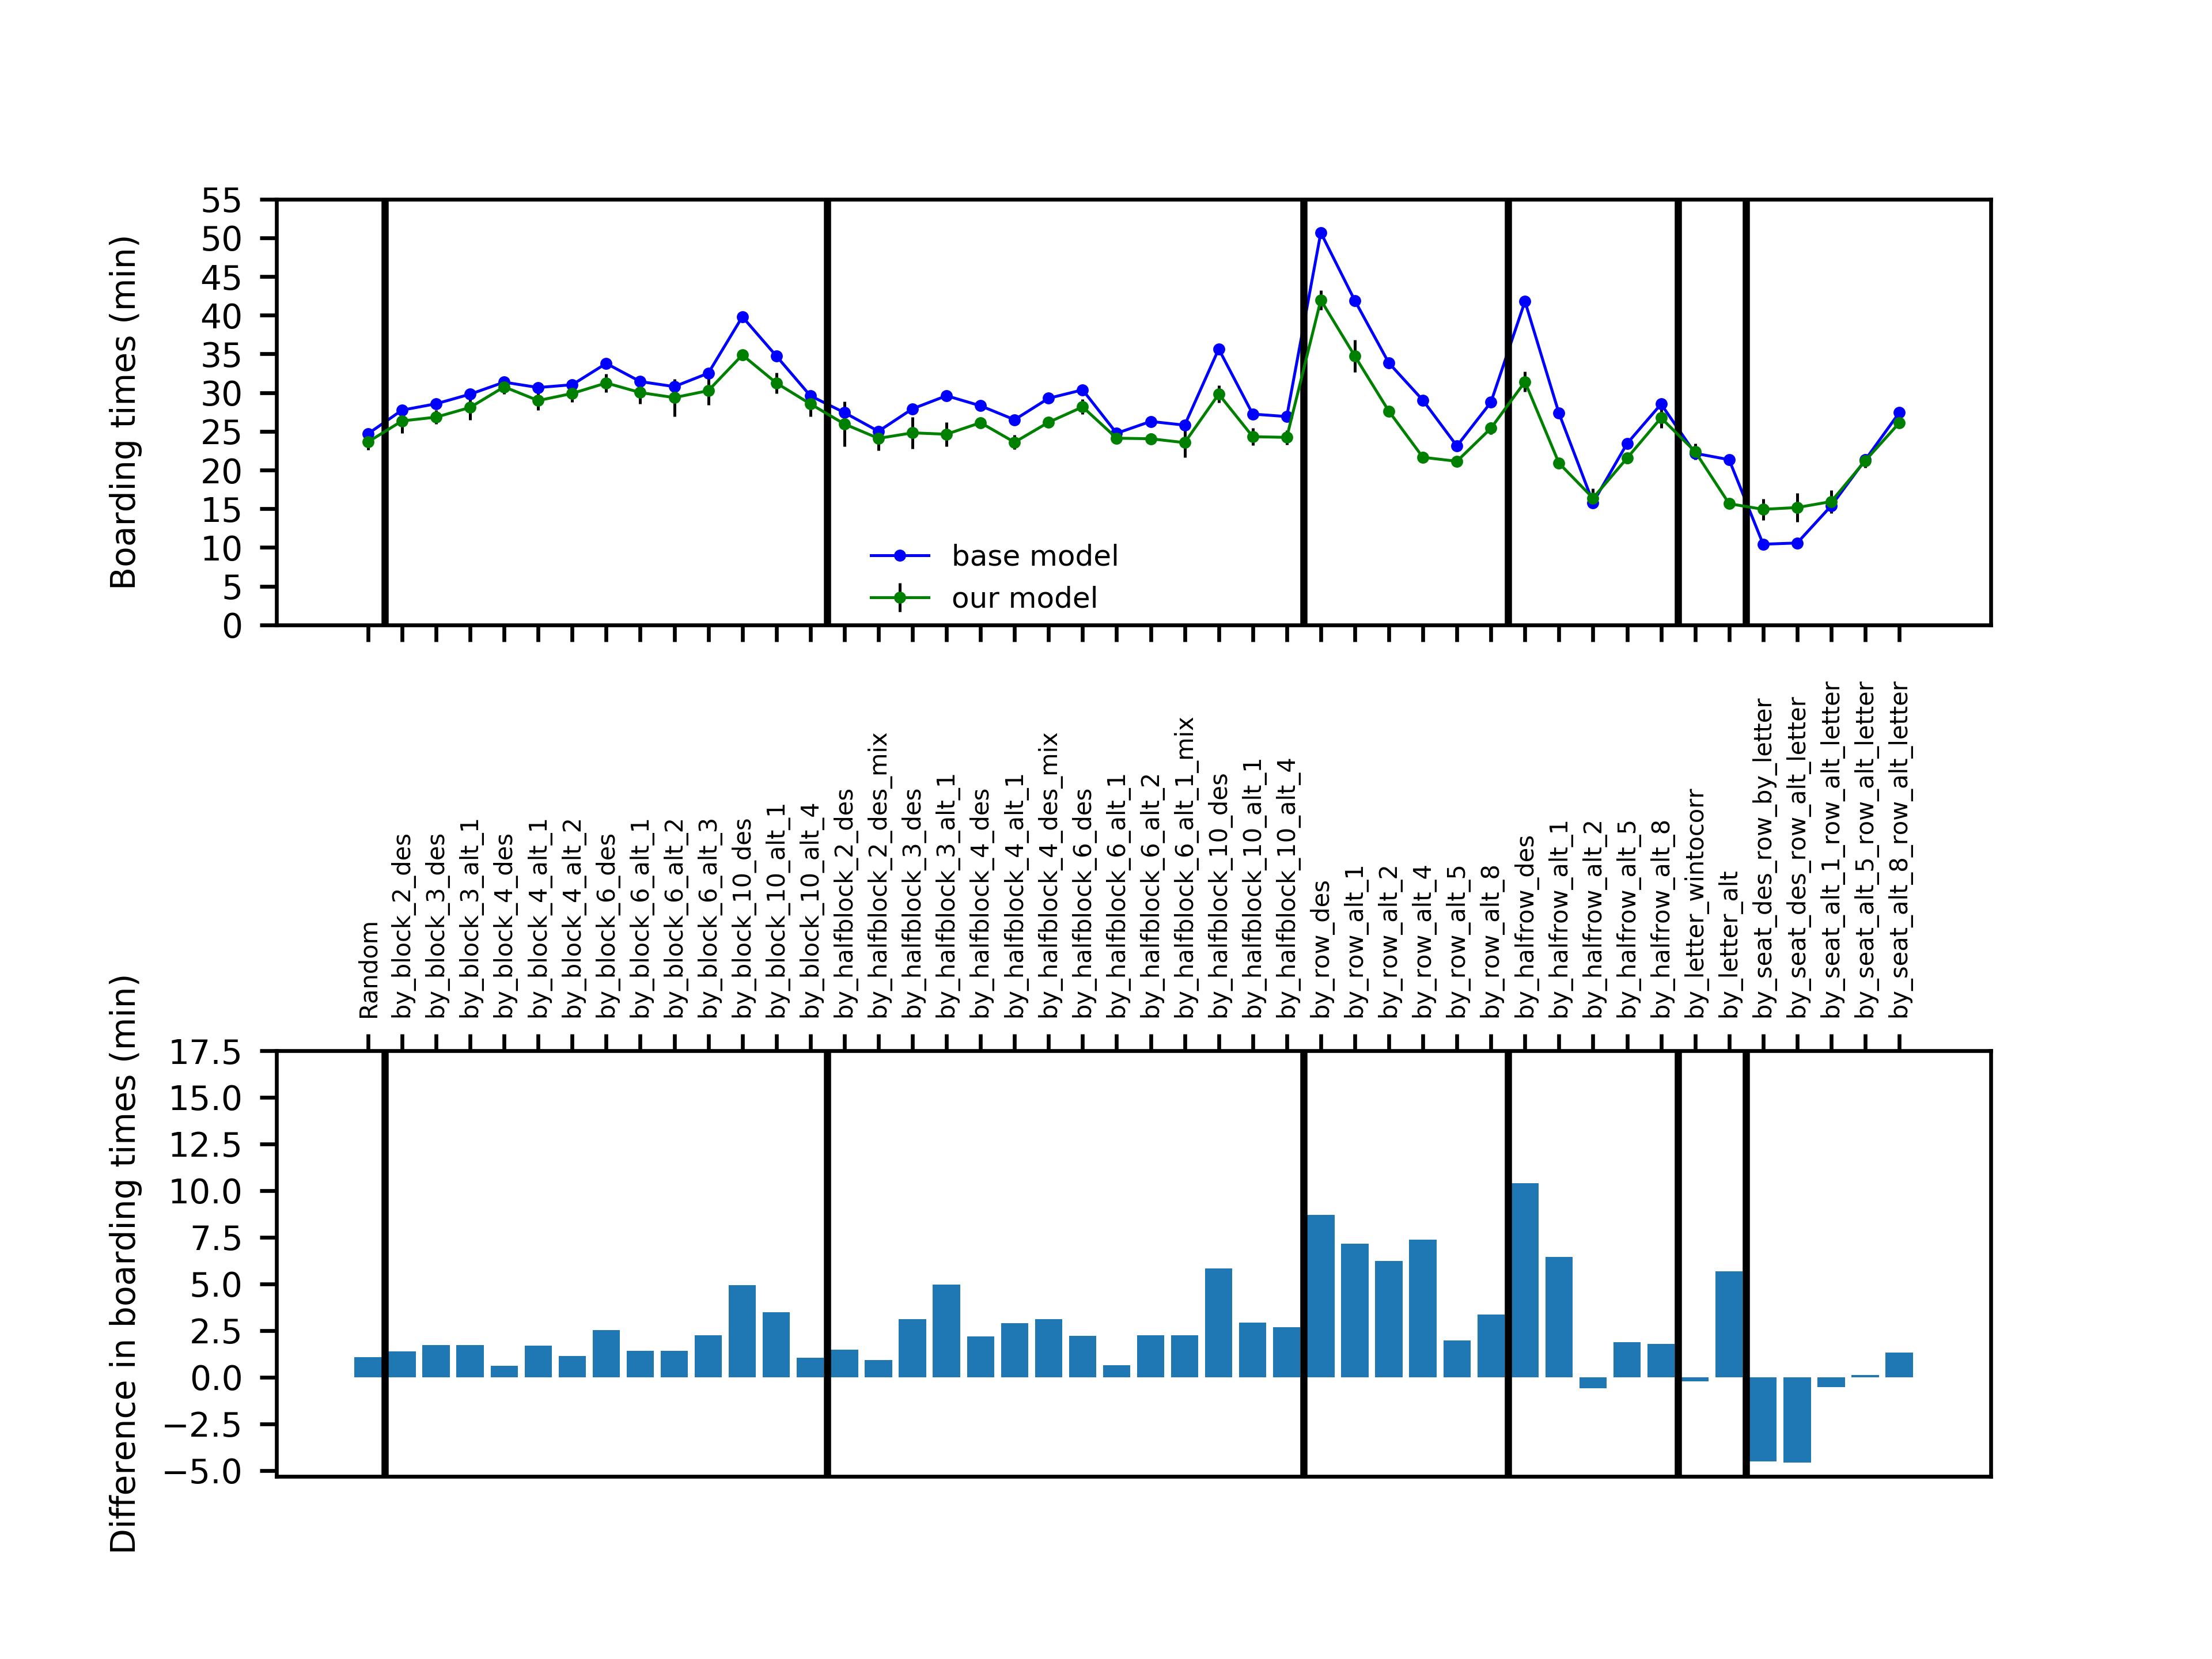
\includegraphics[width=\linewidth]{../../code/AirplaneBoarding/data/figure1/figure1.png}
	\caption{This figure compares the results from our model, using a similar airplane and load specifications, to the ones from the model used in \cite{beus}.}
	\label{figure1}
\end{figure}
\subsection{Result Comparison - Our model vs. Van Landeghem's and Beuselinck's Model}
In order to validate the correctness of our model we compare the different boarding times resulting from employing the same boarding methods as was done in \cite{beus} with a similar airplane and load level. The airplane used in both models are equivalent in the number of rows they have (23) and the number of seats in each row (6), with the only minor exception that the plane they used only had 3 seats in the first and last row. However this difference is very minor, so we decided to neglect it. The passenger load level, so the percentage of occupied seats in the aircraft, are in both cases identical at $100\%$. Furthermore the luggage load level in the simulation from Van Landeghem and Beuselinck was set to normal, which we had to translate into the percentage of occupied overhead compartment space, as our model handles luggage differently to theirs. We believe that when the plane is completely booked out, it is reasonable to assume that $90\%$ of available overhead compartment space is occupied with a normal load level.

In total for each of the 46 boarding methods (excluding method "by\_block\_B-E" because it differentiates with business class in addition to economy class, which, for given reasons, we don't do) we performed 5 trials, in order to have a small sample to calculate the mean time taken for each boarding method within a $95\%$ confidence interval.
The results for the confidence intervals of the total boarding times and differences to Van Landeghem's and Beuselinck's results (their minus our) are displayed in Figure \ref{figure1}. For numerical values, please check table \textit{Insert reference here} in the Appendix.
Analysing the results lead to following conclusions:


The first conclusion that can be drawn is that the average boarding times for our model are generally lower with only a few exceptions. This phenomenon is most likely caused by the different ways the two models handle luggage. In our model the time it takes to store luggage inside a specific compartment does not increase with the amount of luggage that is already inside, which is the case for the other model. Furthermore, not everyone necessarily has any luggage with them because the number of actors (138) is much larger than the total amount of hand-luggage (75) distributed between them (no one more than 2 pieces), which means there are plenty which can directly move to their seat. In the case of the other model, every actor has between 1 and 3 pieces of luggage, so in total almost at least twice the amount of carry-on luggage and there is no one without any. These two aspects further support the results. On the other hand, compartments can be full, not allowing any more actors to store any of his carry-on inside of it, which means those actors have to find other free spots, which takes time and can cause interferences.  To what extend each of these aspects impacts the result can not be said as we have not enough information about the model used in \cite{beus}. 
	
The two exceptions to this observations occur in the class "by\_seat", but only with the two that do not alternate between rows. The reason for that is most likely that the actors in our model first always try to store their luggage in the overhead compartment above their seat and if possible start storing at the beginning of it, not allowing the actor behind to access the same compartment. So if actors that are right behind each other in the boarding sequence have seats in the same or adjacent rows, they might obstruct one another when they both have hand-luggage. This is would also explain why the exception is only seen in the two methods within class "by\_seat" that do not alternate between rows, so adjacent actors in the boarding sequence have adjacent rows. This attribute of the actors only negatively impacted the difference in time in one class because in all the others we look at larger groups, which are random within, and not at individual seats and arrange those. Because the exception to the phenomenon, that the times of our model are generally lower, only occurs in those two methods and is caused by something reasonable, the validity of our model is not impacted. 

Now, in order to be able to conclude that our model is at least as valid as the one used by Van Landeghem's and Beuselinck's, we need to evaluate the impact that the found phenomenon has. 

First of all, the general trend of the data is retained by our model because within each class, especially the larger ones, the difference in boarding times is fairly constant, which again can be seen in the bottom diagram of Figure \ref{figure1}. 


\section{Summary and Outlook}

\section{References}
\begin{thebibliography}{9}
	\bibitem{beus}
	Van Landeghem, H, and A Beuselinck. 
	\textit{"Reducing Passenger Boarding Time in Airplanes: A Simulation Based Approach."} 
	European Journal of Operational Research, vol. 142, no. 2, 2002, pp. 294–308.,
	doi:10.1016/s0377-2217(01)00294-6.
	
	\bibitem{nasa}
	Data Passenger Size from:  NASA. “Man-Systems Integration Standards.” Man-Systems Integration Standards, vol. 1, July 1995, p. 30.
\end{thebibliography}





\end{document}  



 
